\section{Theoretische Grundlage}
\label{sec:Theorie}

\subsection{Einführung}
Ist in einem Raum keine Materie vorhanden und der Gasdruck verschwunden, wird dieses als perfektes Vakuum bezeichnet. Bereits die griechischen Philiosophen Ende des 4. Jahrhunderts konnten die Gedankenspiele über die Existenz eines leeren Raums nicht zweifelsfrei beantworten. Mit dem Aufstreben der Quantenmechanik, stellt sich erneut die Frage in wie fern überhaupt ein teilchenfreier Raum in den Grenzen der Energie-Zeitunschärfe möglich ist, worauf im Folgenden noch eingenangen wird. Rein phänomenologisch ist das Vakuum definiert als:

``\textit{Vakuum heißt der Zustand eines Gases, wenn in einem Behälter der Druck des Gases und damit die Teilchenzahldichte niedriger ist als außerhalb oder wenn der Druck des Gases niedriger ist als 300 mbar, d. h. kleiner als der niedrigste auf der Erdoberfläche vorkommende Atmosphärendruck}'' \cite{DIN}

Ziel des Versuches ist es die Grundlagen der Vakuumtechnik nachzuvollziehen und die für den Versuch benötigten Komponenten kennenzulernen. Dies geschieht indem für die beiden verwendeten Pumpenarten das Saugvermögen, als auch eine Leckratenmessung durchgeführt wird.

\subsection{Messgrößen zur Bestimmung des Vakuums}
Das Maß eines Vakuums ist der Druck $p$. Dieser ist definiert als Kraft $F$ pro Fläche $A$
\begin{equation}
  p = \frac{F}{A} = \left[ \frac{\text{N}}{\text{m}^2} \right]
  \label{eqn:druck}
\end{equation}
Anhand dessen lässt sich das Vakuum in verschiedene Kategorien unterteilen, was im späteren noch passieren wird. Desweiteren lässt sich bei einem Gemisch aus Gasen der Gesamtdruck $p_\text{Ges}$ in mehrere Partialdrücke aufteilen. Es gilt, dass die Summe über alle Partialdrücke dem Gesamtdruck entspricht. Analog wird mit der Teilchenanzahl vorgegangen. Der Partialdruck entspricht dem Druck welcher das entsprechende Gemisch in dem selben Volumen, wodrin sich $p_\text{Ges}$ befindet ausüben würde. \newline
Der Druck wird üblicherweise in den Einheiten mbar gemessen. Der Normaldruck ist auf 1013 mbar definiert. 1 bar Entspricht in etwa $10^{5}$ Pa. \newline
Desweiteren zeichnet sich ein Gas durch die mittlere freie Weglänge $\Lambda$ eines Teilchens aus, bis es mit einem anderen wechselwirkt. Durch einführen eines Stoßquerschnitts und bei einer konstanten Teilchenzahldichte $n$ lässt sich durch lösen einer Differentialgleichung
\begin{equation}
  \frac{dN}{N} = -n \sigma \Delta x
  \label{eqn:mfWDGL}
\end{equation}
zeigen, dass die mittlere freie Weglänge  inversproportional zu dem Produkt aus Teilchenzahlichte und Stoßquerschnitt ist.
\begin{equation}
  \Lambda = \frac{1}{n \sigma}= \frac{k T}{\sqrt{2} \pi D^2 p}
  \label{eqn:mfW}
\end{equation}
Da die Teilchenanzahl von Luft bei Normaldruck als gegeben vorrausgesetzt wird, kann aus der Vorraussetzung, dass das Produkt aus $p\cdot V$ konstant ist, die Teilchenzahl bei den anderen Drücken berechnet werden.
\begin{table}
  \centering
  \caption{Übersicht über die Druckbereiche, die mittlere freie Weglänge und die Teilchenanzahl}
  \begin{tabular}{c|c c c}
  	\toprule
	Druckbereiche & Druck / mbar & Moleküle / $cm^3$ & mittlere freie Weglänge \\
	\midrule
	Normaldruck	& 1013.25			& $2.7 \cdot 10^{19}$ &	68 nm \\
	Unterdruck	& > 300				& k.A. & k.A \\
	Grobvakuum	& 300 \ldots 1 			&$10^{19} \cdot 10^{16}$&0.1 \ldots 100 $\mu m$ \\
	Feinvakuum	& 1 \ldots $10^{-3}$		& $10^{16} \cdot 10^{13}$ & 0.1 \ldots 100 mm \\
	Hochvakuum	& $10^{-3} \cdots 10^{-7}$	& $10^{13} \cdot 10^{9}$ & 100 mm \ldots 1km \\
	Ultrahochvakuum	& $10^{-7} \cdots 10^{-12}$	& $10^9 \cdots 10^4$ & 1 m \ldots $10^5$ m \\
	extrem hohes Vakuum & $< 10^{-12}$		& $<10^4$ & $> 10^5$ \\
	\bottomrule
  \end{tabular}
  \label{tab:ueberblick}
\end{table}
\subsection{p(t) Kurve}
Für die Auswertung wird eine Funktion benötigt welche den Druck in abhängigkeit der Zeit angibt. Dafür muss die Annahme getroffen werden, dass die Saugleistug $S$ für den angegebenen Zeitraum konstant ist und nicht vom Druck $p(t)$ abhängt. Dann entspricht die zeitliche Änderung des Volumens
\begin{equation}
  \frac{\text{d}V}{\text{d}t} = S \ .
\end{equation}
Zusätzlich wird eingefordert, dass die Temperatur des Gases bei dem Vorgang konstant ist. Mithilfe des idealen Gasgesetzes
\begin{equation}
  p V = n R T
\end{equation}
lässt sich für eine zeitabhängige Druckänderung
\begin{equation}
  \frac{\text{d}}{\text{dt}} pV = \frac{\text{d}}{\text{dt}} n R T
\end{equation}
bei konstanter Stoffmenge $n$ im System die Gleichung
\begin{equation}
  \frac{\text{d}p}{\text{d}t} V= \frac{\text{d}V}{\text{d}t} p
  \label{eqn:konti}
\end{equation}
herleiten. Durch lösen der DGL ergibt sich die Gleichung:
\begin{equation}
  p(t) = p_0 \exp \left( \frac{-t}{\tau} \right)
\end{equation}
Durch einsetzen der Anfangsbedingungen und des Enddrucks $p_\text{E}$ ergibt sich für den Zeitabhängigen Druck
\begin{equation}
  p(t) = (p_0 - p_\text{E}) \exp \left( -t \frac{S}{V} \right) + p_\text{E}
  \label{eqn:Druck}
\end{equation}
\subsection{Bestimmung des Saugvermögens über die Leckratenmessung}
Das Saugvermögen $S$ ist gleich dem Quotienten aus des Leckrate des Rezipienten $Q$ und dem Gleichgewichtsdruck $p_\text{g}$.
\begin{align}
   S = \frac{Q}{p_\text{g}}
\end{align}
Die Leckrate $Q$ ergibt sich zu
\begin{align}
   Q = V_0\, \frac{\Delta p}{\Delta t}
\end{align}
Aus dem Volumen $V_0$ des Rezipienten und dem Quotienten $\frac{\Delta p}{\Delta t}$ lässt sich das Saugvermögen der Pumpe bestimmen, wenn die Zeit $t$ gegen den Druck $p$ aufgetragen wird. Daraus folgt für das Saugvermögen
\begin{align}\label{eqn:SaugLeck}
   S = \frac{V_0}{p_\text{g}}\, \frac{\Delta p}{\Delta t}
\end{align}
\subsection{Wechselwirkungsprozesse Restgas Umgebung}
Befindet sich ein Gas oder eine Flüssigkeit eingeschloßen in einem Körper, wechseltwirkt das Gas oder die Flüssigkeit mit der Grenzfläche. Dabei können die aufgeführten Prozesse auftreten und die Messreihe beeinflussen. In Kapitel \ref{sec:Durchführung} werden Maßnahmen vorgestellt dem entgegenzuwirken. (Föhnen, Rezipient verschließen).
\begin{itemize}
  \item \textbf{Absorption:} Trifft ein Teilchen auf die Grenzfläche, kann es passieren das es von dieser aufgenommen wird. Dannach befindet es sich für unbestimmte Zeit im Absorbermaterial, kann jedoch auch wieder reduktieren.
  \item \textbf{Adsorption:} Trifft ein Teilchen auf die Grenzfläche kann es sich neben der Absorbtion auch am Rand des Absorbermaterials ablagern. Dabei wird es mittels der Van-der-Waals Kräfte am Rand lokalisiert.
  \item \textbf{Desorption:} Es ist der Umkehrprozess der Absorbtion. Dabei wird ein Teilchen aus dem Rezipienten an das Vakuum abgegeben und ist somit nicht mehr lokalisiert.
  \item \textbf{Diffusion:} Ist in einem geschlossenen System eine inhomogenen Gasverteilung, sorgt die Diffusion dafür, dass die Verteilung in den Gleichgewichtszustand über geht. Es beruht darauf das die ungerichteten Bewegungen die Zeitumkehrinvarianz brechen und das System in den Zustand der maximalen Entropie treibt.
  \item \textbf{Ausgasen:} Ist ein Festkörper durch zu langen kontakt mit der Umwelt verureinigt, muss bei diesem die Gasteilchen zunächst ersteinmal an die Oberfläche diffundieren bevor sie desobiert werden können. Dadurch kann nicht so schnell der Sättigungswert für die Pumpen erreicht werden.
\end{itemize}
\subsection{Strömungsprozesse und Leitwert}
Bewegungen von Fluiden werden meist durch Schichten beschrieben. Dabei sind Oberflächenphänomene und der Verlauf der Schichten von besonderem Intresse.
\subsubsection{Laminare Strömung:}
Als laminare Strömung wird eine turbulenzfreie Strömung verstanden. Dabei mischen sich die Schichten von Flüssigkeiten, wenn sie an Hindernissen vorbeifließen, nicht untereinander.

\subsubsection{Molekulare Strömung:}
Als molekular Strömung wird eine Strömung bezeichnet, wenn ihre mittlere freie Weglänge größer ist, als der Durchmesser der Strömung. Dies passiert immer dann, wenn die Drücke hinreichend klein (typisch wären Hoch-/Ultrahochvakuum) sind. Aufgrund der geringen Teilchendichte wechselwirken diese öfters mit den Grenzflächen als untereinander.

\subsubsection{Leitwert:}
Zur Berechnung des Saugvermögens einer Pumpe wird der Strömungswiderstand der Geometrie des Aufbaus berücksichtigt. Dafür wird der Quotient aus der Länge der Leitung und des Strömungswiderstandes gebildet.
\begin{equation}
  C = \frac{l}{W} = \frac{q_\text{pV}}{\Delta p}
\end{equation}
Der Strömungswiderstand verhält sich analog zum elektrischen Widerstand. Dementsprechend sind die Kirchhoffschenregeln ebenso gültig.

\section{Technische Grundlagen}
Im Folgenden werden die für den Versuch benötigten Technischen Grundlagen skizziert.
\subsection{Pumpentypen und Funktionsweise}
Pumpen lassen sich anhand der verschiedenen Saugraten $S$, ihrer Funktionsweise und den erreichten Enddrücke $p_\text{E}$ kategorisieren. Eine Übersicht über die verschiedenen Pumpen kategorisiert nach deren funktionsweisen ist in Abblidung \ref{fig:Uebersicht} zu sehen.
\begin{figure}[htbp]
  \centering
  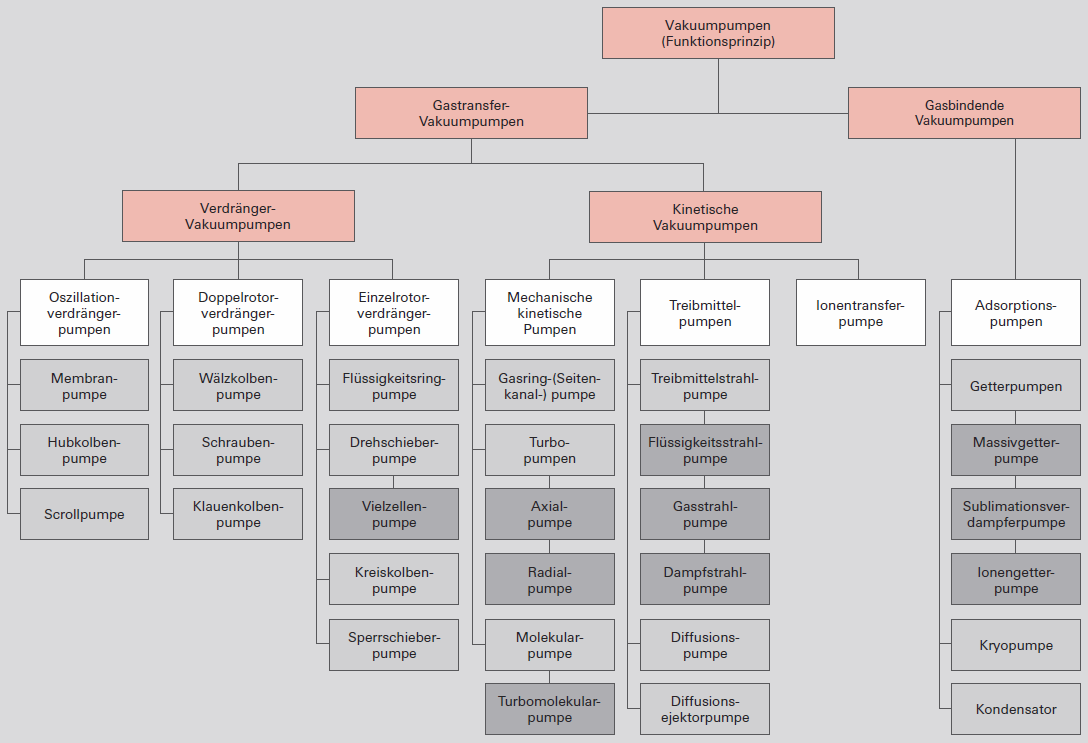
\includegraphics[width=0.9\textwidth]{picture/Uebersicht.png}
  \caption{Übersicht der verschiedenen Kategorien von Vakuumpumpen \cite{Uebersicht}}
  \label{fig:Uebersicht}
\end{figure}
Die funktionsweise von kinetische Pumpen beruht darauf, dass durch Beschleunigung des Gases in Pumprichtung der Gasdruck verringert wird.
Verdrängerpumpen kennzeichen sich dadurch aus, dass aufgrund von Volumenvergrößerungen der Gasdruck gesenkt wird.
Gasbindenende Pumpen zeichnen sich dadurch aus, dass Sie die Gas-Moleküle an der Oberfläche des Rezipienten binden und somit den Druck senken. Sie werden manchmal auch als Speicher-Pumpen bezeichnet, weil Sie die Moleküle nicht abtranspotieren, sondern an der Oberfläche des Rezipienten lokalisieren. Mit ihnen lassen sich nach Einstellung eines Vorvakuums sehr geringe Drücke herstellen.
Allgemein lassen sich alle Pumpen die Gas aus dem Rezipienten an die Umgebung transportieren als Transportpumpen zusammenfassen.
Beispielhaft werden drei Pumpen vorgestellt, welche weit verbreitet in der Vakuumstechnik sind.
\subsubsection{Drehschieberpumpe:}
\begin{wrapfigure}{r}{0.32\textwidth}
    \vspace{-1cm}
    \centering
    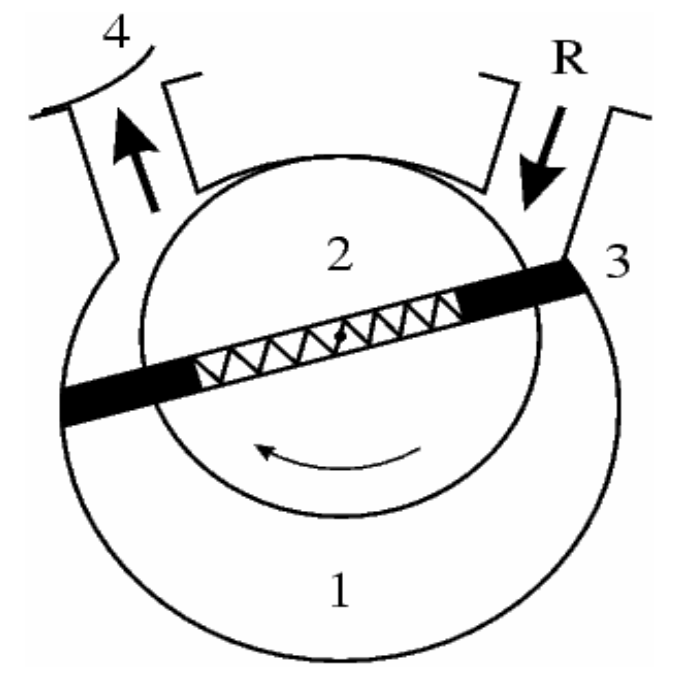
\includegraphics[width=0.3\textwidth]{./picture/Drehschieberpumpe.png}
    \caption{Querschnitt \cite{Dreh},\cite{Jena}}
    \label{fig:Dreh}
\end{wrapfigure}
Die Drehschierbepumpe ist eine Verdrängerpumpe und eine Skizze vom Aufbau ist in Abbildung \ref{fig:Dreh} abgebildet. Sie kennzeichnet sich durch eine zylindrische Kammer aus wodrin ein zylindrischer Rotor gelagert ist. An dem Rotor befinden sich zwei Drehschieber welchen den Inhalt der Drehkammer in zwei Volumina aufteilt. Die Zylinderische Kammer ist einerseits mit dem Rezipient und andererseits mit der Außenwelt verbunden. Durch die Volumenvergrößerung des Rezipienten strömt Gas in die Pumpe, welches durch ein Überdruckventil durch kompression nach einem halben Rotorumschlag das Gas an die Umwelt abgibt. Der Enddruck $p_\text{E}$ ist im wesentlichen durch das Restvolumen bestimmt, wenn die Luft gerade beim Auslass komprimiert wird. Drehschieberpumpen haben typischerweise eine Saugleistung von einigen Litern. Der Enddruck befindet sich im Bereich von hPa.
\subsubsection{Turbomolekularpumpe:}
\begin{wrapfigure}{l}{0.35\textwidth}
    \vspace{-1cm}
    \centering
    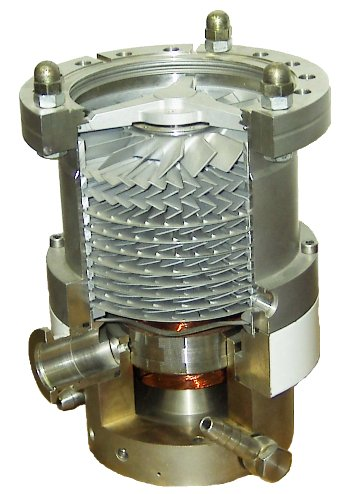
\includegraphics[width=0.33\textwidth]{./picture/Turbo.jpg}
    \caption{Querschnitt Turbopumpe \cite{Turbo}}
    \label{fig:Turbo}
    \vspace{-0.5cm}
\end{wrapfigure}
Die Turbopumpe benötigt für die inbetriebnahmen ein Vorvakuum und gehört zu den kinetischen Pumpen. Sie zeichnet sich durch ihren abwechselnden Aufbau aus Turbinen und Statorscheiben aus. Die Ventilatorblätter sind gegen die Scheibenebene gekippt und haben nach außen hin ein immer größer werdenden Neigungswinkel. Fällt ein Gas-Molekühl aus dem Rezipienten auf die Turbinenflügel wird dieses kurz von diesen Absorbiert, Adsorbiert bzw Stößt mit diesen und wird anschließend weiter zu den Rotorblätter mit einem höheren Neigungswinkel durchgereicht. Damit die Turbopumpe arbeiten kann, muss die mittlere freie Weglänge der Gasmoleküle in der Größenordung des Abstandes der Rotorblätter oder größer sein. Die Turbomolekularpumpe erzeugt typischerweise Enddrücke von bis zu $10^{-6}$ mbar. Bei Drehzahlen von einigen 10.000 Umdrehungen pro Minute erreichen Turbomolekularpumpen je nach Geometrie Saugleistungen von mehreren Litern bis zu tausenden von Litern.

\subsubsection{Ionengetter-Pumpe}
Die Ionengetterpumpe gehört zu dem Bereich der Sorptionspumpen. Das Wirkungsprinzip beruht darauf das die Gasteilchen ionisiert werden und anschließend mittels eines angelegten Feldes zum Gettermaterial befördert werden. Somit ist dieses an der Oberfläche des Gettermaterials gebunden und verringert den Druck effektiv im Volumen des Rezipientens welches keinen Kontakt zur Grenzfläche besitzt. Durch thermische Prozesse lässt sich in gewissen Grenzen die beschränkte Aufnahmefähigkeit des Gettermaterials erhöhen. Daher ist es von Intresse beim Einsatz ein gutes Hochvakuum zu besitzen. Mit der Ionengetter-Pumpe ist es möglich Drücke von bis zu $10^{-11}$ mbar zu erzeugen.

\subsection{Messgeräte}
Für die Messung von verschiedenen Drücken werden unterschiedliche Messinstrumente benötigt. Jedes hat ihren eigenen Arbeitsbereich und muss daher zur vollständigen Beobachtung der Erzeugung eines Hochvakuums ausgehend vom Normaldruck entsprechend in den Versuchsaufbau gebaut werden. Desweiteren muss gewährleistet werden, dass die Geräte beim erzeugen des Vakuums keinen Schaden nehmen. Die Messgeräte werden im folgenden sortiert nach ihrem Wirkungsbereich von Normaldruck zum Vakuum vorgestellt und ihre Funktionsweise kurz erläutert.

\subsubsection{Pirani Messgerät}
\begin{wrapfigure}{l}{0.5\textwidth}
  \centering
  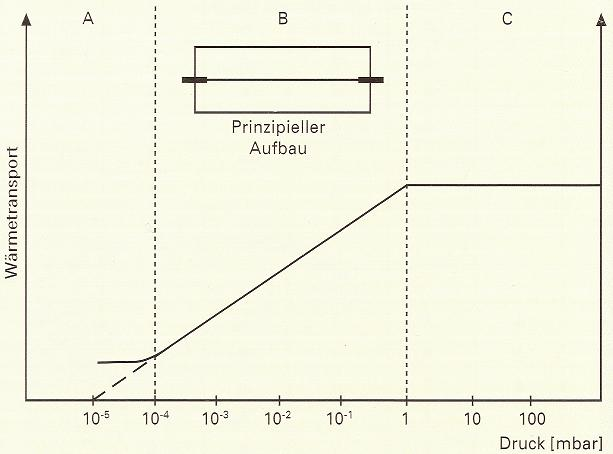
\includegraphics[width=0.48\textwidth]{picture/Pirani.JPG}
  \caption{Abhänigkeit der Wärmekapazität vom Druck \cite{Dreh}, \cite{Jena}}
  \label{fig:pirani}
  \vspace{-0.6cm}
\end{wrapfigure}
Das Pirani Messgerät bei denen die druckabhängige Wärmeleitung des Gases ausgenutzt wird, kommt bei Drücken zwischen Normaldruck und 50 nbar zum Einsatz. Die Wirkungsweise beruht darauf, dass in dem genannte Gebiet, wie in Abbildung \ref{fig:pirani} zu sehen, die Wärmeleifähigkeit proportional zum Druck ist. Das technische Prinzip beruht darauf, dass ein Draht durch einen konstanten Strom geheizt wird und dieser seine Wärme über statistische Prozesse an die sich in dem zu messenden Körper befindlichen Teilchen abgibt. Somit ist die Temperatur des Gases mit dem spezifischen Widerstand des Stromes korreliert. Wird nun der Strom gemessen, kann nach einer Eichung der Druck gemessen werde. In den Bereichen A und C der Abildung \ref{fig:pirani} ist die Wärmeleitfähigkeit nicht mehr proportional zum Druck. In gewissen Maßen lassen sich jedoch noch Drücke oberhalb von 1 mbar abschätzen, jedoch liegt dem Messprinzip ein anderes physikalisches Prinzip zugrunde.

\subsubsection{Kaltkathoden-Messgerät}
Beim Kaltkathoden-Messgerät wird ein großes E-Feld angelegt, welches Primär-Elektronen, welche von der natürlichen Raumionisation stammen, abzieht. Aufgrund der Beschleunigung durch das Feld, ionisieren die Primär-Elektronen weitere Gasmoleküle, sodass der Strom vergrößert wird. Dieser Effekt wird durch Anlegung eines äußeren B-Feldes verstärkt, da dadurch die Elektronen aufgrund der Lorentz-Kraft auf Kreisbahnen gezwungen werden und der Weg zur Anode hin anwächst. Durch Messung des Ionisationsstrom kann auf den Druck rückgeschlossen werden, jedoch muss berücksichtigt werden das der Strom auch von der Gasart abhängig ist. Der Messbereich des Kaltkathodenmessgerätes ist nach unten hin bis ca $10^{-4}$ mbar beschränkt, da trotz der verlängerten Messtrecke nicht genügend Gasmoleküle ionisiert werden.

\subsubsection{Heißkathoden-Messgerät}
\begin{wrapfigure}{r}{0.3\textwidth}
  \vspace{-1.0cm}
  \centering
  \includegraphics[width=0.28\textwidth]{picture/Heißkathode.png}
  \caption{Funktionsweise Heißkathoden-Messgerät \cite{Heiss}}
  \label{fig:Heißkathode}
  \vspace{-1cm}
\end{wrapfigure}
Die Wirkungsweise des Heißkathoden-Messgerät ähnelt dem des Kaltkathoden-Messgerät stark. Dadurch das es jedoch bei niedigeren Drücken zum einsatz kommt, werden zu wenig Elektronen durch die natürlichen Raumionisation frei. Aufgrund dessen wird eine Glühkathode genutzt welche Elektronen freisetzt welche auf dem weg zur Anode Gasmoleküle ionsieren. Durch Messung des Ionenstroms kann somit der Druck bestimmt werden. Der Messbereich ist nach oben bis ca $10^{-2}$ mbar beschränkt, weil sonst die Glühkathode beschädigt wird und nach unten bis ca $10^{-9}$ mbar.
\section{Fehlerrechnung}
Sämtliche Fehlerrechnungen werden mit Hilfe von Python 3.4.3 durchgeführt.
\subsubsection{Mittelwert}
Der Mittelwert einer Messreihe $x_\text{1}, ... ,x_\text{n}$ lässt sich durch die Formel
\begin{equation}
	\overline{x} = \frac{1}{N} \sum_{\text{k}=1}^\text{N} x_k
	\label{eqn:ave}
\end{equation}
berechnen. Der Fehler des Mittelwertes beträgt
\begin{equation}
	\Delta \overline{x} = \sqrt{ \frac{1}{N(N-1)} \sum_{\text{k}=1}^\text{N} (x_\text{k} - \overline{x})^2} \ .
	\label{eqn:std}
\end{equation}

\subsubsection{Gauß'sche Fehlerfortpflanzung}
Wenn $x_\text{1}, ..., x_\text{n}$ fehlerbehaftete Messgrößen im weiteren Verlauf benutzt werden, wird der neue Fehler $\Delta f$ mit Hilfe der Gaußschen Fehlerfortpflanzung angegeben.
\begin{equation}
	\Delta f = \sqrt{\sum_{\text{k}=1}^\text{N} \left( \frac{ \partial f}{\partial x_\text{k}} \right) ^2 \cdot (\Delta x_\text{k})^2}
	\label{eqn:var}
\end{equation}
